\documentclass[paper=a4, fontsize=12pt]{article} % A4 paper and 11pt font size
\usepackage[T1]{fontenc} % Use 8-bit encoding that has 256 glyphs
\usepackage[english]{babel} % English language/hyphenation
\usepackage{amsmath,amsfonts,amsthm} % Math packages
\usepackage{a4wide}
\usepackage{float}
\usepackage{longtable}
\usepackage{hyperref}
\usepackage{listings}
\usepackage{makecell}
\usepackage{graphicx}
\usepackage[table]{xcolor}
\usepackage[numbered, framed]{mcode}  % To load matlab code
\lstset{deletestring=[b]{"}}

\usepackage{fancyhdr} % Custom headers and footers
\pagestyle{fancyplain} % Makes all pages in the document conform to the custom headers and footers
\setlength\parindent{0pt}
\fancyhead[L]{SF3565, Project 3, November 2016}
\fancyhead[R]{H{\"a}ggmark, Karlsson} % Empty left footer
\fancyfoot[C]{Program construction in C++ for Scientific Computing} % Empty center footer
\fancyfoot[R]{\thepage} % Page numbering for right footer

\title{Program construction in C++ for Scientific Computing \\ Teacher: Michael Hanke}

\author{Ilian H{\"a}ggmark \\ mail \href{mailto:ilianh@kth.se}{ilianh@kth.se}
  \and Andreas Karlsson \\ mail \href{mailto:andreas.a.karlsson@ki.se}{andreas.a.karlsson@ki.se} }
\date{\normalsize\today} % Today's date or a custom date

\begin{document}

\maketitle % Print the title

\section*{Project 3}
\subsection*{Task 1 - Abstract Class}

The class \texttt{Curvebase} is created to hold basic functionality for curves, but not the curves them-self. The class has therefore functions \texttt{x} and \texttt{y} that calls the derived classes that contain the specific curve information. The grid generation for which the class will be used should not know about specifics either so the \texttt{Curvebase} is a kind of interfaces that convert a normalized position on a curve ( zero to one) to the actual position that the grid point generation requires. The functions \texttt{x} and \texttt{y} will thus take the normalized arc length parameter $s$ and return \texttt{xp}$(p)$ and \texttt{yp}$(p)$ respectively. The functions \texttt{xp} and \texttt{yp} are pure virtual function (i.e. must be implemented in the derived class) that return \texttt{x} and \texttt{y} values given $p$ which is the actual position on the curved. Before calling \texttt{xp} and \texttt{yp} Curvebase must calculate $p$ from $s$. This is done by solving the equation 

$$ \texttt{fp}(p) = \ell(p)- s\cdot  \ell(b) = 0 $$

where 

$$ \ell (p) = \int_a^p \sqrt{\texttt{dxp}(q)^2+\texttt{dyp}(q)^2} \textrm{d}q $$

a and b are the upper and lower bounds of the curve and \texttt{dxp} and \texttt{dyp} are the derivatives of \texttt{xp} and \texttt{yp}. $\ell ()$ gives the length and $\ell (b)$ thus the total length of the curve. Newton's equation is used to solve the first equation.\\

The function \texttt{fp()} in \texttt{Curvebase} is used to calculate $p$ with Newton's methods. This is performed many times and the efficiency should be considered. \texttt{fp()} needs the total length of the curve, $\ell (b)$. This can be done by calling integrate. Doing this every time \texttt{fp()} is called is however not smart since the length of a curve is constant. We therefore want to create a variable in the \texttt{Curvebase} that contains the length. \texttt{Curvebase} is however an abstract class an does no know anything about the curve. We solve this by declaring a length variable in \texttt{Curvebase} an the initializing the variable in the constructor of the inherited class. Setting length as a variable gives an decrease in computational time by a factor $\sim 2.5$\\



\subsection*{Task 2 - Curve Generation}

The derived curve objects are quite simple since most of the machinery lies in the abstact class. The derived object mainly holds two important things: the limits of the curve ($a$ and $b$) and the description of the curve in terms of the functions \texttt{xp}, \texttt{yp}, \texttt{dxp}, and \texttt{dyp}. These functions simple contain the mathematical description of the curves.

\subsection*{Task 3 - Domain Class}

The most important part in terms of efficiency for this project is the nested loop that calculated gridspoints inside the \texttt{generate\_grid()} function. The expresstion used to calculate the $x$ coordinate (for $y$-term $x$ is simply exchanged for $y$) from the nommalized arc length parameter $s$ is

\begin{align*}
x[j+i*(m\_+1)]  &= \varphi_1(ih_1)\cdot \textrm{sides}[3]->x(jh_2) \\
	&+ \varphi_2(ih_1)\cdot \textrm{sides}[1]->x(jh_2) \\
	&+ \varphi_1(ih_2)\cdot \textrm{sides}[0]->x(ih_1) \\
	&+ \varphi_2(jh_2)\cdot \textrm{sides}[2]->x(ih_1) \\
	&- \varphi_1(ih_1) \varphi_1(jh_2) \cdot  \textrm{sides}[0]->x(0) \\
	&- \varphi_2(ih_1) \varphi_1(jh_2) \cdot  \textrm{sides}[1]->x(0) \\
	&- \varphi_1(ih_1) \varphi_2(jh_2) \cdot  \textrm{sides}[3]->x(1) \\
	&- \varphi_2(ih_1) \varphi_2(jh_2) \cdot  \textrm{sides}[2]->x(1)
\end{align*}

The four last term are corner correction terms. Calculating this expression $(m\_+1)(n\_+1)$ times it very inefficient since the calling calculating the $x$-function of a side is computationally heavy. We can however reduce the number of calls. The $\varphi$-function are very small and can be left as they are (inlining gives little improvement). We should however lift out the parts that contain the call to sides.$x()$. We note that the ``sides'' part of the four corner terms does not depend on $i$ and $j$. It is thus extremely inefficient to calculate them for every loop iterator. We can simply calculate them once before the loop starts. We also note that the first four lines are calculated $(m\_+1)(n\_+1)$ times even though $(m\_+1)$ times or $(n\_+1)$ times would be enough. We do this by calculating the first two lines in one loop and storing them in a vector, then doing the same thing for the 3rd and 4th line. The nested loop that finally puts everything together will thus not contain one call to the heavy $x$-function. This gives totally a decrease in computational time by a factor $\sim 2n_$. Generating one milion grid points took e.g. $2.5$ seconds on an average Intel dual core processor.  \\

\subsection*{Task 4 - Data Exportation}

The vectors \texttt{x\_} and \texttt{y\_} are concatenated before they are saved with
the code given in the task. The produced file can then be read and
visualized, as can be seen in Figure \ref{fig:grid}, using
the \textsc{Matlab} code below.

\begin{lstlisting}
  fid = fopen('outfile.bin','r'); % Open file
  c = fread(fid,'double');        % load file content to vector c

  x = c(1:length(c)/2);           % first half of c is x values
  y = c(length(c)/2+1:end);       % second half of c is y values

  plot(x,y,'.')                   % plot the x,y points
  \label{lst:matlab}.
\end{lstlisting}

\begin{figure}[H]
  \centering
  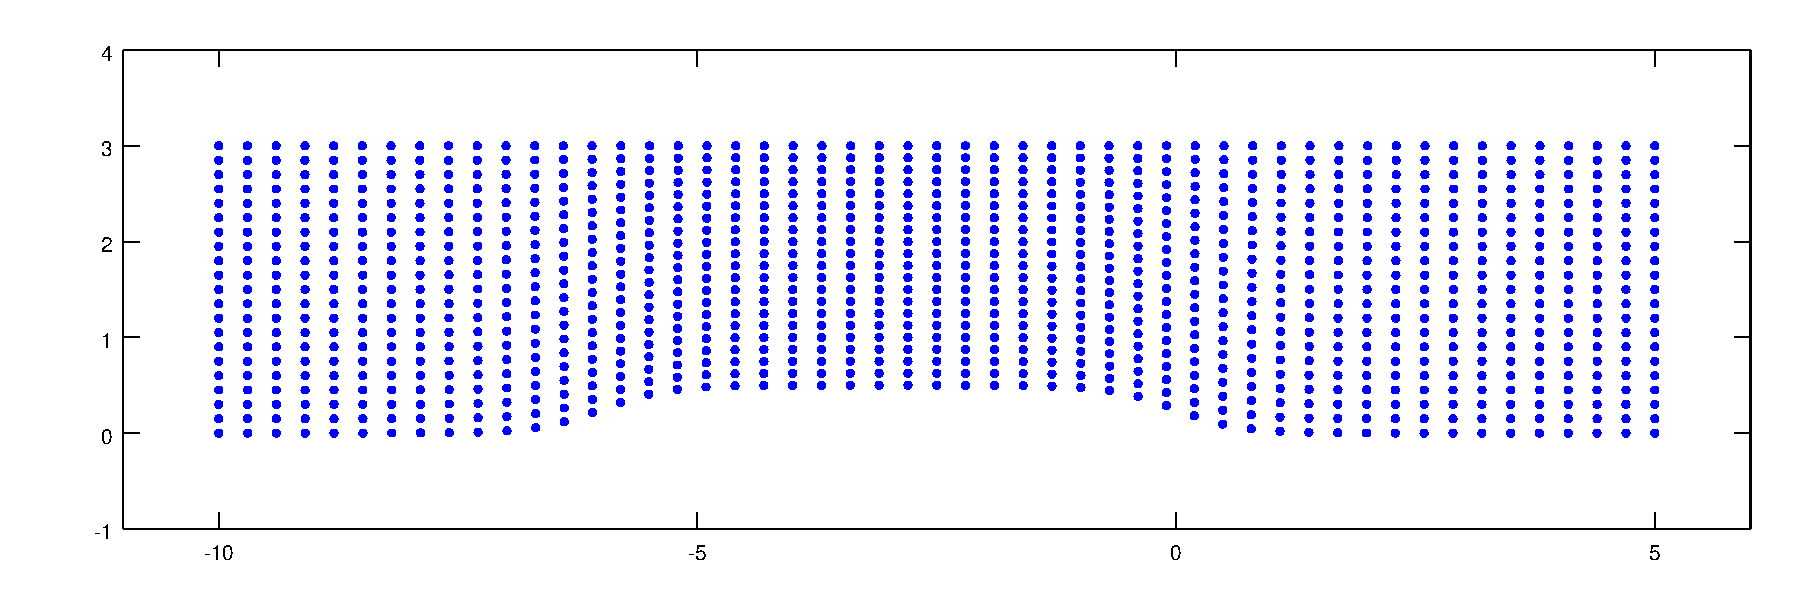
\includegraphics[width=\textwidth]{task4.pdf}
  \caption{Grid produced by the \texttt{generate\_grid()} method and plotted with \textsc{Matlab.}\label{fig:grid}}
\end{figure}

\subsection*{Task 5 - Grid stretching}


\begin{figure}[H]
  \centering
  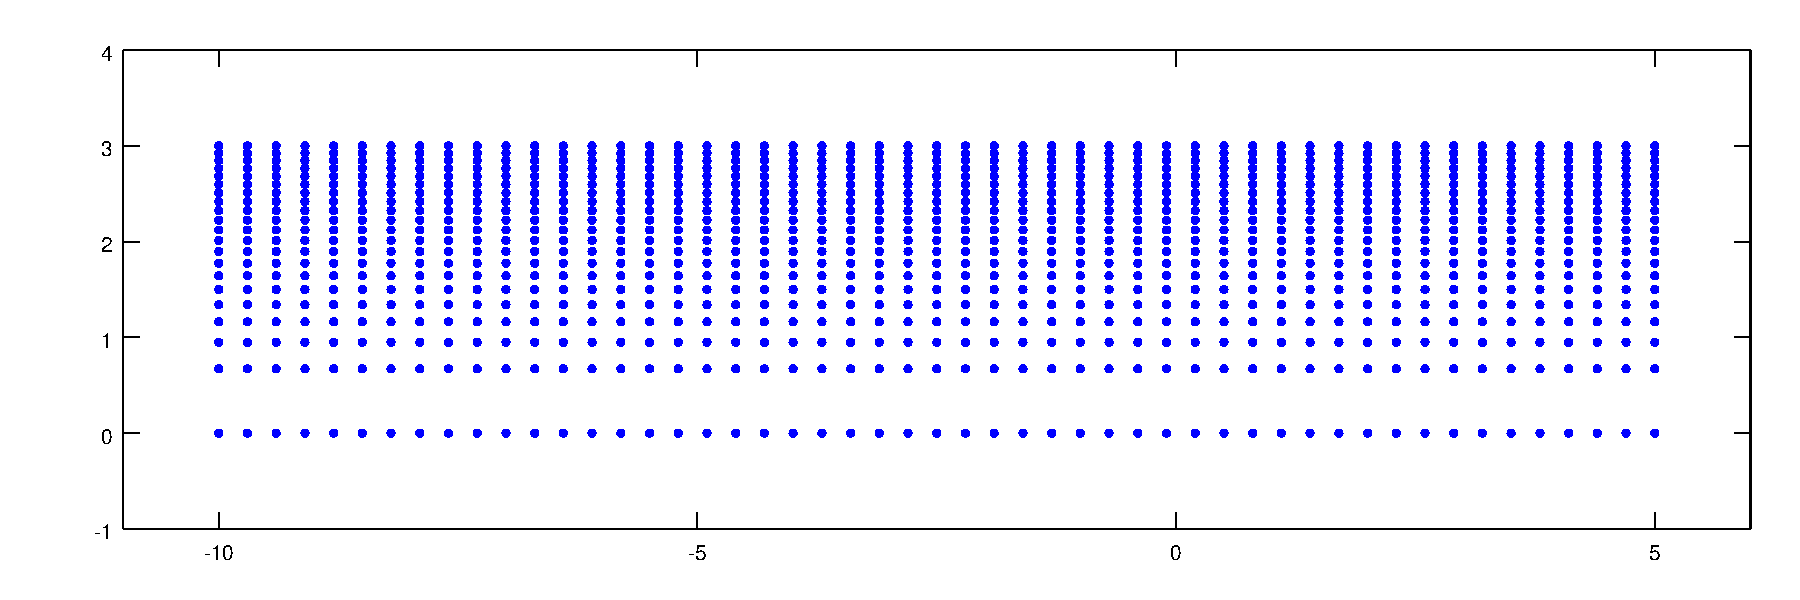
\includegraphics[width=\textwidth]{task5.pdf}
  \caption{A stretched grid plotted with \textsc{Matlab.}\label{fig:stretched}}
\end{figure}

We added an (optional) boolean argumnet in the generate_grid function. When true the expression given in task 5 was appiled to $j*h_2$ in the calls to the function \texttt{y} in \texttt{Curvebase}. This stretch the grid in the vertical direction, while still not changing the boundries (as expected).  

\end{document}
